% !TeX root = ../main.tex
% Add the above to each chapter to make compiling the PDF easier in some editors.

\chapter{Stereo Rendering Optimization - Input reduction}
When looking at real-time rendering as it is done today - albeit from a strongly simplified perspective - the CPU could be described as a employer and the GPU as an employee. For each frame, the CPU produces certain render tasks and supplies the necessary information such as draw calls, shader parameters, buffers and so forth. The GPU then consumes these tasks and associated items and dos the heavy lifting to produce the required results. 
Now if one wants to speed up that overall process, there are two major ways. One way is to reduce the amount of data that is put into the pipeline so less data needs to be processed overall, the other way is to increase the efficiency of the processing itself.  
This first chapter of optimization approaches presents ways of reducing the amount of data or work input. 

\subsubsection{(Hierarchical) Frustum culling}
The following options build on top of the regular frustum culling concept. In this the objects in the scene are checked against a camera frustum whether they are inside or outside of it or intersecting with the surface of the frustum. The checks themselves can be generally optimized in various ways, regardless of whether stereoscopy is desired or not. Often only an object's bounding geometry is checked, collections of objects can be precomputed so larger numbers may be discarded at once. An advanced option of culling is to delegate the calculations into a GPU compute shader so potentially less data needs to be transferred from the CPU per frame and much higher vector/matrix calculation is gained in exchange for slower branching. Some modern renderers also do very granular culling like bitmasked checks of precomputed triangle sets, as seen in Ubisoft's Anvil Next engine used in Assassin's Creed Origins\cite{Haar.2015}. 
Another optional layer of the culling process is to maintain hierarchical container structures for the scene objects so larger numbers can be discarded or included early on. 
For all those options the goal is the same, to get as result the list or buffer of objects visible by the given camera frustum in the scene. 

\subsubsection{Frustum culling in Tachyon}
The frustum culling approach in Tachyon is fully CPU-based and utilizes pre-computed hierarchical draw buffers. More specifically, at startup the scene is divided into a coarse grid of \codeword{chunk}s where each grid possesses an octree. Also at startup, a thread pool with the current number of hardware threads is created. At asset load time, these octrees are populated with the loaded objects through optimistic size-aware insertion. Each cell of a tree then precomputes a draw buffer containing a combined draw call for all objects associated with that cell. These buffers can be recomputed at any time, but the operation should be avoided at runtime as it incurs costly CPU to GPU transfers. 
In a culling pass, first all \codeword{chunk}s within a certain draw distance radius of the camera are chosen, so there is an additional very primitive distance culling taking place. Then each \codeword{chunk} submits a culling call using its tree to the thread pool. Each such call works as follows: \\

\textcolor{red}{[TODO: brief rundown of SceneChunk::FrustumCull] \\}

One problematic area remains, however, and that is Z ordering. Modern graphics pipelines will perform early Z discard during the fragment stage. If a fragment fails the depth test for a given draw call, meaning its geometry would be occluded by triangles already written to the fragment, the shader will skip any further calculation for this geometry and fragment. For this to take hold in performance improvement, the draw calls need to be issued in a manner where geometry closer to the camera is drawn first. If draws are done in reverse order, the pipeline will draw distant geometry first and subsequent closer geometry at the same fragment will naturally not fail the depth test and overwrite the fragment. Effectively, all prior writes to any such fragment in that frame would be wasted and go unseen. This issue is called overdraw and can significantly deteriorate GPU render times in extreme cases. 
One such example would be the following, very dense synthetic test scene: \\

\textcolor{red}{[TODO: image of scene with high object density and distance] \\}

If the draw calls for each populated octree cell are issued back to front, the overdraw of many dozens if not hundreds of layers can push frametimes to 300 milliseconds and beyond on the test machine, while issuing the calls front to back results in frametimes of 11 milliseconds or less. 
This stark contrast in performance highlights the importance of good Z ordering. 

\textcolor{red}{[TODO: Put the following in or not? \textit{At this time, rtvklib does not successfully employ such call reordering. A conservative and thus only moderately beneficial front to back ordering is in the works but due to the nature of the octree cells' pre-recorded command buffers, overdraw cannot be avoided without a significant rewrite of these pre-recordings.}]}

\section{Superfrustum Culling}
\subsection{Theory}
The basic idea behind Superfrustum culling is to essentially do regular frustum culling despite rendering into two cameras, one per eye. The naive way of extending the frustum concept to a stereoscopic camera is to add a second frustum so there is one per eye, then perform the culling check for both frusta and merge the results. \\
As is easily visible from \textcolor{red}{[TODO: illustration of stereo frusta]} though, the spatial proximity of of these two frusta leads to a large overlap volume, especially as field of view increases with more advanced headsets. One possible strategy to leverage more performance when culling two eyes is a so-called Superfrustum, assuming the frustum is the common six sided trapezoid. Cass Everitt of Facebook LLC, formerly Oculus LLC \textcolor{red}{[TODO: check correct corp names]} has suggested this approach and provided computation sketches on his social media back in 2015 \cite{Everitt.2015}(\autoref{fig:Everitt_Superfrustum}), and Nick Whiting at Oculus Connect 4 teased it as a future addition to Unreal Engine 4 \cite{Whiting.2017}. The idea is to combine the left and right eye frusta by taking the respective widest outer FOV tangent - usually the left eye's right side and the right eye's left side - and using these as the new side tangents of the superfrustum. Another way to express these is to take the widest half opening angles of each eye and adding them up to a combined opening angle. Similar is done for the top and bottom tangents, although these will usually be nearly identical for the two eyes. \\
A pitfall of the superfrustum is its necessary depth recession. This is easy to visualize when combining the two frusta by extending aforementioned side tangents backwards until they cross. The meeting point of this step is the new origin of the superfrustum, slightly recessed behind the two separate eyes. 
Vivien Oddou of Silicon Studios offered a generalized way to compute this recession for non-mirrored eye orientation\cite{Oddou.23.05.2017}, while Everitt has extended his sketches by an asymmetry normalization\cite{Everitt.2015b}. Both of these are important to consider as virtual reality headsets can have slightly canted and asymmetrical lenses, either by design or by manufacturing tolerance. Ignoring these two corrections may still result in a sufficient superfrustum if computed conservatively, but should be included for fully correct setups. 
While this superfrustum naturally eliminates all overlap of the naive variant, it in turn includes small false positive regions, notably the triangular void found close to the origin points between the two eye frusta and potential side edge regions in the case of asymmetrical lens orientations. In a typical application, the performance cost of these will be negligible. \\

\begin{figure}[htb]
  \centering
  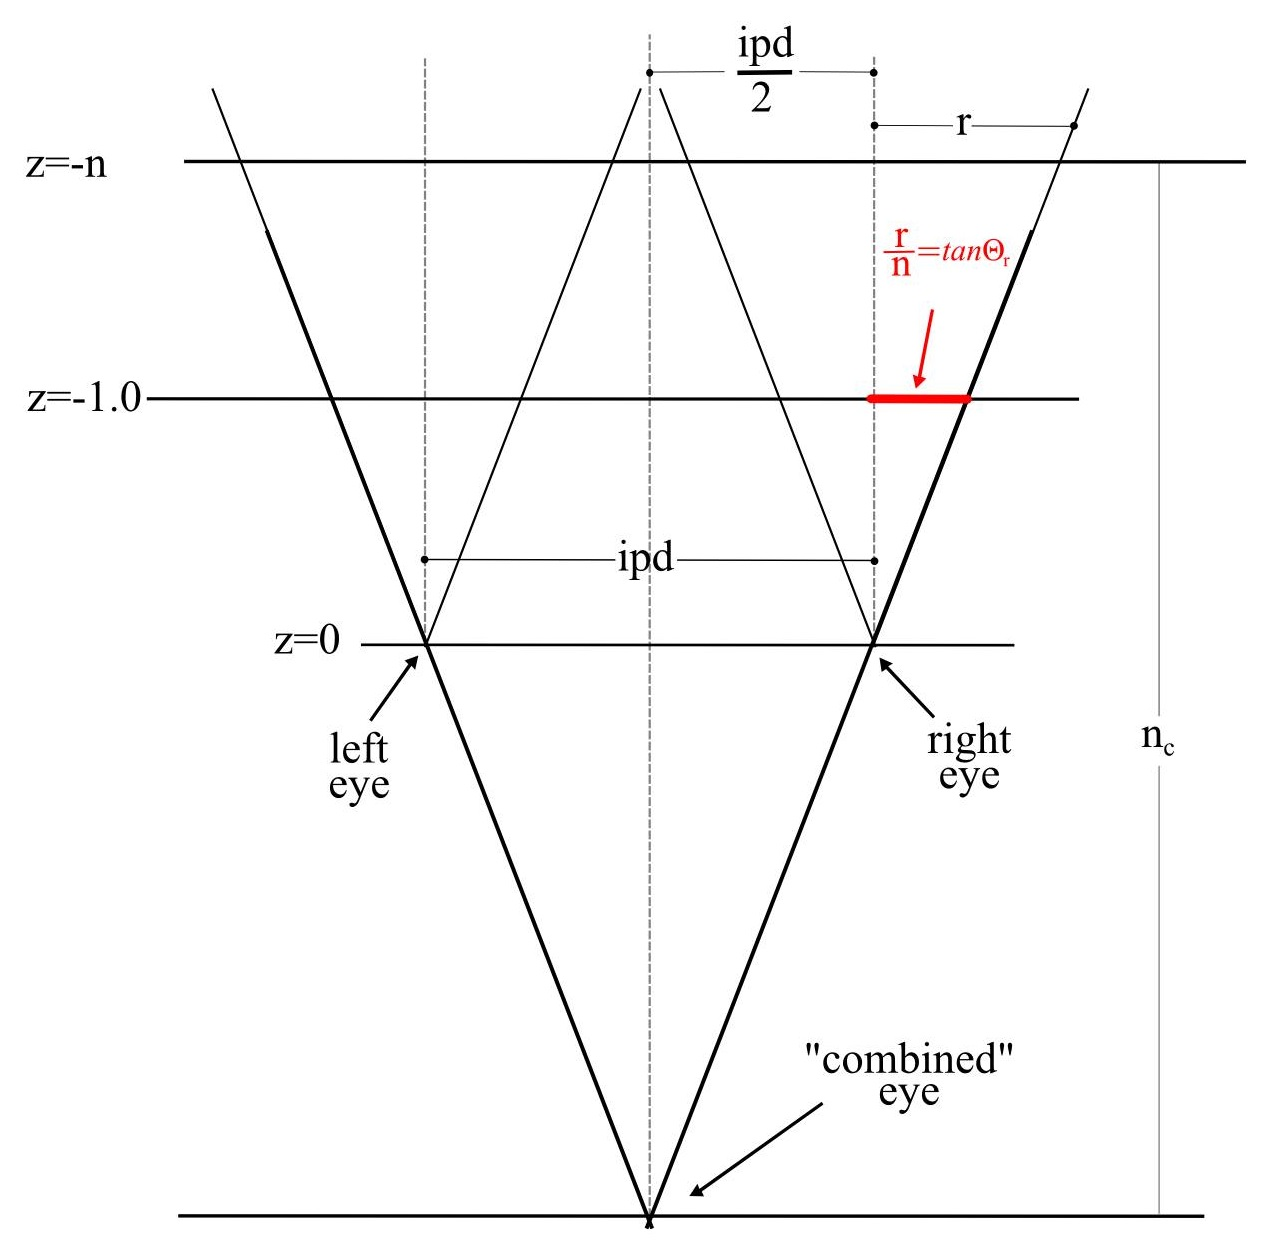
\includegraphics[width=0.7\textwidth]{pictures/Everitt_Superfrustum_Crop}
  \caption{Symmetric Superfrustum (cropped to geometric construction)\cite{Everitt.2015}} \label{fig:Everitt_Superfrustum}
\end{figure}

\subsection{Estimated impact}
The impact of using a Superfrustum will depend very specifically on the type of frustum culling done and combination with other techniques. \\
On its own with a CPU based culling pass only an appreciable benefit in CPU rendering time is to be expected as the number of frustum checks will be reduced by up to 50\% and only a single buffer needs to be transferred to the graphics unit. The GPU itself still needs to render each eye separately though, including all vertex transformations, pixel shading and so forth. The specific impact in the case of Tachyon is elaborated on in \autoref{results}. \\
Superfrustum culling when performed directly on the GPU obviously has great potential to significantly cut down on related compute work, once again to the effect of up to 50\% versus a baseline dual frustum culling. An interesting point to consider is whether any of the culling data needs to be synchronized back to the CPU, as when not, the GPU compute workload will only depend on a single small buffer or pushconstant transfer containing the camera parameters. If, however the resulting culling set is transferred back to the CPU, for example for preprocessing of the next frame, this transfer will of course present another speedup limiter. 

\subsection{Implementation specifics}
To facilitate Superfrustum culling in Tachyon required only straight-forward changes. At creation time of the virtual camera, the superfrustum is computed from the given OpenVR eye parameters following Everitt and Silicon's way, outlined in \textcolor{red}{[TODO: pseudo code]}. 
The calculated superfrustum recession and new combined field of view angles are saved and used every frame when re-transforming the superfrustum. The frustum transformation uses a simple geometric approach where the camera's world position, forward and up vectors in conjunction with the near and far distance, field of view and aspect ratio are extruded into the six planes of the frustum volume. 
The per-frame culling pass of Tachyon then naturally only checks against this single frustum and returns a single set of draw commands that are then sent to both eyes. 



\section{Round Robin Culling}
Another culling variant specific to stereoscopy uses the round robin principle. The concept again springs from the desire to avoid frusta overlap, but instead of combining the frusta, it exploits a common property of current stereoscopy rendering techniques. As modern headsets use circular lens optics and flat displays distorting the displayed image, the framebuffers commonly need to be warped to compensate so the picture looks undistorted to the user again. As a result a lot of the edge data of the image is either considerably squeezed together or outside of the visible area of the HMD displays.
This conservative property means a virtual eye frustum can be smaller than the technical frustum of that respective eye and false negative discards in these edge regions would go unseen by the user.
Assuming both eyes of the headset have similar opening angles and parallel or nearly parallel viewing direction, the overlap of the two frusta would in most cases encompass the entire stereo-visible volume. So it naturally follows that only culling for one of the eye frusta would already give a sufficient representation of the actually visible scene. \\

However, there is still a possibility of missing a few edge cases with this alone. So the extension of the idea to actual round robin assumes another common property of modern VR headsets, namely high refresh rates. Many of these aim for at least 80Hz (Rift S, WMR) ranging up to 144Hz (Index experimental mode) image refresh to give the user a smooth visual sensation.
Exactly halving that refresh rate and reprojecting images for two refresh cycles with some pixel interpolation is an established way to still provide an acceptable experience with minor visual artifacting on slower devices as demonstrated by Oculus LLC's Asynchronous Space Warp \textcolor{red}{[TODO: and/or Time Warp?]} and SteamVR's reprojection features. It follows that a conceivable compromise is to alternate which frustum is used for culling in a round robin fashion so that even if edge cases include visible false negatives, they only persist for one frame at a time. In the worst case this would manifest as shimmering or flickering at the outer edges of the visible screen area. \\
Overall this makes Round Robin Culling a viable candidate on systems with very limited culling performance, but the tight constraints for sufficiently accurate results make it unfit as a general recommendation. \\

\textcolor{red}{[TODO: small illustration?]}



\section{Conical Frustum Culling}
This third alternative culling extension targets the circular shape of HMD lenses for leverage. Coming back to the conservative framebuffer size from the previous section, the lenses lead to a lot of invisible area in the corners of the display. Jonathan Hale attempts to demonstrate the method in his thesis \cite{Hale.2018} as both a contribution to the graphics middleware \textit{Magnum}\cite{Vondrus.30.10.2019} and a UE4 extension at Vhite Rabbit\cite{VhiteRabbit.08.01.2020} - albeit with limited success. That proof of concept does show the validity of the method though. The traditional six sided trapezoid frustum is replaced by a cone encompasses a volumetric projection of the view through each respective lens. For a more geometry-bound GPU, this method will provide a small relief. \\

\textcolor{red}{[TODO: more specific description of approach from paper]
[TODO: small illustration]}

\subsubsection{Merging approaches}
A convenient side effect of these three presented optimizations is that they can in part be merged. It is conceivable, for example, to do Conical Round Robin Frustum Culling in an effort to slice away as much of the conservative invisible area as possible and reduce the list of drawable objects to an optimistic minimum. It is also possible to construct a Conical Superfrustum aiming to avoid the mentioned edge false positives, albeit only feasible if the display per eye is square-like to avoid adding new false positive volume on other sides.
